\documentclass[a4paper,12pt]{article}

%% Language and font encodings
\usepackage[english]{babel}
\usepackage[utf8x]{inputenc}
\usepackage[T1]{fontenc}

%% Sets page size and margins
\usepackage[a4paper,top=2cm,bottom=2cm,left=3cm,right=3cm,marginparwidth=1.75cm]{geometry}

%% Useful packages
\usepackage{amsmath}
\usepackage{mathtools}
\usepackage{graphicx}
\usepackage{bigstrut}
\usepackage{numprint}
\usepackage{color}
\usepackage{float}
\usepackage[figurename=Figura]{caption}
\usepackage[tablename=Tabella]{caption}

\title{Edit Distance e N-grammi}
\author{Lorenzo Pesci}
\date{5 Luglio 2020}

\begin{document}
\maketitle

\section{Introduzione}
Vogliamo analizzare le differenze tra Edit Distance e N-grammi dato un lessico $L$ e una stringa $Q$ per trovare le parole in $L$ più vicine a $Q$.

Entrambe sono tecniche che determinano quanto due stringhe siano simili.

Vengono utilizzate per la correzione di parole isolate, per correggere documenti, per suggerire query all'utente e per correzione di documenti antichi tramite OCR.

\subsection{Edit Distance}
La distanza di edit tra due stringhe $A$ e $B$ è il numero minimo di modifiche elementari che consentono di trasformare la $A$ nella $B$. Per modifica elementare si intende:
\newline
- la cancellazione di un carattere \newline
- la sostituzione di un carattere con un altro \newline
- l'inserimento di un carattere \newline
- la copia di un carattere \newline
- lo scambio tra due caratteri vicini

\subsection{N-grammi}
Il problema con l'Edit Distance è il grande numero di confronti da effettuare con un dizionario.

Una possibile soluzione è utilizzare l'intersezione di n-grammi, ovvero enumerare tutti gli n-gram in $Q$ e il $L$, usare un indice di n-gramma per trovare tutti i termini in $L$ che contengono "abbastanza" n-grammi di $Q$.

La distanza tra due stringhe è calcolata tramite il \textbf{coefficiente di Jaccard}, definito come la dimensione dell'intersezione divisa per la dimensione dell'unione degli n-grammi ($J(A,B) = \frac{|A \cup B|}{|A \cap B|}$).

Nel nostro caso, $A$ e $B$ sono insiemi di n-grammi.
Dalla definizione si può vedere che il coefficiente di Jaccard è compreso tra 0 e 1 ($0<J(A,b)<1$).

In particolare, il coefficiente è zero se $A$ e $B$ sono disgiunti ed è 1 se A e B hanno gli stessi elementi.

\subsection{Considerazioni teoriche}
Per come sono stati implementati, sia l'Edit Distance che gli N-grammi sono metodi che scorrono un'intero dizionario.
La differenza sostanziale tra le due consiste nel numero di operazioni svolte per ogni parola: l'$edit\_distance$ esegue molte più operazioni di $ngram$ poichè gli n-grammi sono stati calcolati a parte.

\clearpage
\section{Analisi delle Operazioni di Edit Distance}

Nella nostra trattazione useremo le seguenti notazioni:
\newline
- X e Y sono le stringhe da confrontare \newline
- M e N sono le rispettive lunghezze \newline
- c matrice dei costi \newline
- op matrice delle operazioni \newline
- i e j sono indici che vanno da 0 a m-1 e da 0 a n-1, utilizzati per scorrere matrici \newline
- t tabella utilizzata per immagazzinare i costi delle operazioni ottime

\subsection{edit distance(x, y)}
La funzione $edit\_distance$ è un algoritmo che, prese in ingresso due stringhe, costruisce le matrici $c$ ($M \times N$) e $op$ ($M \times N$). $C$ rappresenta la matrice di costi associata alle operazioni descritte nella matrice $op$, necessarie per convertire la stringa $X$ nella stringa $Y$.

\subsection{op sequence(op, i, j, t)}
La funzione $op\_sequence$ è un algoritmo ricorsivo che, presa in ingresso la matrice delle operazioni (restituita da $edit\_distance$), gli indici i e j (inzialmente m-1 e m-1) e la tabella t (inizialmente vuota), riempie t con le operazioni migliori da utilizzare nella trasformazione.
La funzione restituisce il valore di ritorno della funzione $calc\_cost$.

\subsection{calc cost(t)}
La funzione $calc\_cost$ è un algoritmo che, presa in ingresso la tabella t, restituisce un intero $c$ che è la somma dei costi delle operazioni in t (trovate grazie a $op\_sequence$).

\section{Analisi delle Operazioni di N-Gram}
Nella nostra trattazione useremo le seguenti notazioni:
\newline
- n è la lunghezza dell'n-gramma \newline
- p è la parola da dividere in n-grammi

\subsection{ngram(p, n)}
La funzione $ngram$ è un algoritmo che, presi in ingresso una parola p e la lunghezza dell'n-gramma n, restituisce un'array contenente gli n-grammi della parola data. (\textbf{Esempio}: $ngram$("algoritmi", 2) ---> ['al', 'lg', 'go', 'or', 'ri', 'it', 'tm', 'mi']).

\subsection{jaccard(ng1, ng2)}
La funzione $jaccard$ è un algoritmo che, presi in ingresso due array contenenti n-grammi qualsiasi (resitituiti da $ngram$), restituisce il coefficiente di Jaccard tra ng1 e ng2.

\clearpage
\section{Descrizione Esperimenti e Documentazione del codice}

Gli esperimenti sono stati svolti su un MacBook Pro con sistema operativo macOS Catalina, processore 2,2 GHz 6-Core Intel Core i7 e 16 GB di RAM.
\newline
\newline
Eventuali numeri casuali sono stati generati dalla funzione \textit{random.randint()} importata dalla libreria \textit{random}.
\newline
\newline
Il codice è articolato in otto file: $edit\_distance.py$, $ngram.py$, $tests.py$, $exp.py$, $save\_ngrams.py$, $60000\_parole\_italiane.txt$, $2\_grams.txt$, $3\_grams.txt$, $4\_grams.txt$.
\newline
\newline
1) Nel file \textbf{edit\_distance.py} è stato implementato l'algoritmo di Edit Distance per il calcolo della distanza tra due stringhe.
\newline
\newline
2) Nel file \textbf{ngram.py} è stata implementata la divisione di una parola in n-grammi e il calcolo del coefficiente di Jaccard dati due n-grammi.
\newline
\newline
3) Nel file \textbf{tests.py} sono stati implementati i seguenti esperimenti (dove non specificato, sono stati utilizzati bigrammi con coefficiente di Jaccard 0.6, e la soglia di Edit Distance è stata impostata a 3):
\newline
\newline
- Presa una parola a caso dal dizionario ($60000\_parole\_italiane.txt$), è stato misurato il tempo impiegato sia con Edit Distance che con N-grammi per trovarla.
\newline
\newline
- Prese 9 parole arbitrarie di lunghezza crescente (['a', 'ad', 'con', 'muro', 'zoppo', 'marito', 'sboccia', 'faticavo', 'abbattete']), è stato misurato il tempo di esecuzione e il numero di parole vicine trovate sia per Edit Distance che per N-grammi.
\newline
\newline
- Presa in input una parola, è stato misurato il numero di risultati trovati al variare della soglia di Edit Distance (1, 2, 3, 4, 5) e del coefficiente di Jaccard (0.5, 0.6, 0.7, 0.8, 0.9).
\newline
\newline
- Prese tre parole casuali di lunghezza $\geq 5$, è stato misurato il numero di parole vicine trovate al variare del numero di n-grammi (2, 3, 4).
\newline
\newline
- Presa una parola in input, essa viene alterata (tramite la funzione $altera(word)$) e viene misurato il numero di risultati trovati al variare della soglia di Edit Distance (1, 2, 3, 4, 5) e del coefficiente di Jaccard (0.5, 0.6, 0.7, 0.8, 0.9). Inoltre si controlla anche se la parola originale è presente tra le parole vicine trovate.
\newline
\newline
4) Nel file \textbf{exp.py} sono stati eseguiti i test descritti nel file \textbf{tests.py}.
\newline
\newline
5) Nel file \textbf{save\_ngrams.py} è stata implementata una funzione che a partire da una lista di 60000 parole ($60000\_parole\_italiane.txt$), genera un file $n\_grams.txt$ (con $2 \leq n \leq 4$) contenente la parola e l'n-gramma corrispondente.

\clearpage
\section{Presentazione Dati Sperimentali}
Vengono di seguito presentati i grafici relativi agli esperimenti svolti:
\newline
\subsection{Tempo di esecuzione Edit Distance e N-grammi}
\begin{center}
\vspace*{0.7cm}
\begin{tabular}{|c|c|c|}
\hline
\textbf{Parola}\bigstrut & \textbf{Tempo edit distance}  & \textbf{Tempo n-gram} \\ \hline
 \textit{elogiavate}\bigstrut & 3.032 & 0.543 \\\hline
 \textit{continuato}\bigstrut & 2.185 & 0.356 \\\hline
 \textit{ammazzero}\bigstrut & 0.578 & 0.112 \\\hline
 \textit{smorzare}\bigstrut & 7.883 & 1.712 \\\hline
 \textit{sequenza}\bigstrut & 6.624 & 1.403 \\\hline
 \textit{assalti}\bigstrut & 0.748 & 0.229 \\\hline
 \textit{ubertose}\bigstrut & 7.404 & 1.731 \\\hline
 \textit{allegavamo}\bigstrut & 0.4385 & 0.1107 \\\hline
 \textit{occupiate}\bigstrut & 4.907 & 0.966 \\\hline
 \textit{espiasti}\bigstrut & 2.549 & 0.5325 \\\hline

\end{tabular}
\captionsetup{justification=centering,margin=1.05cm}
\captionof{table}{Tempo di esecuzione impiegato sia da Edit Distance che da N-grammi per trovare una parola casuale.}
\end{center}

Per questo esperimento sono state prese 10 parole casuali dall'elenco di parole italiane ($60000\_parole\_italiane.txt$).

Per ognuna di esse è stato calcolato il tempo di esecuzione sia per Edit Distance che per N-grammi necessario per trovare la parola data.
\newline
\newline
Dai dati si può notare come l'algoritmo N-grammi sia sempre più rapido rispetto all'Edit Distance nella ricerca delle parole.Questo è dovuto al fatto che nella ricerca di parole N-gram esegue meno operazioni rispetto a edit-distance, la quale si rivela essere molto pesante per la ricerca di parole 'lontane' dall'inizio del dizionario.

\clearpage
\subsection{Tempo di esecuzione di Edit Distance e N-grammi per parole di dimensione variabile}
\begin{figure}[h]
    \centering
    \captionsetup{justification=centering,margin=1.05cm}
    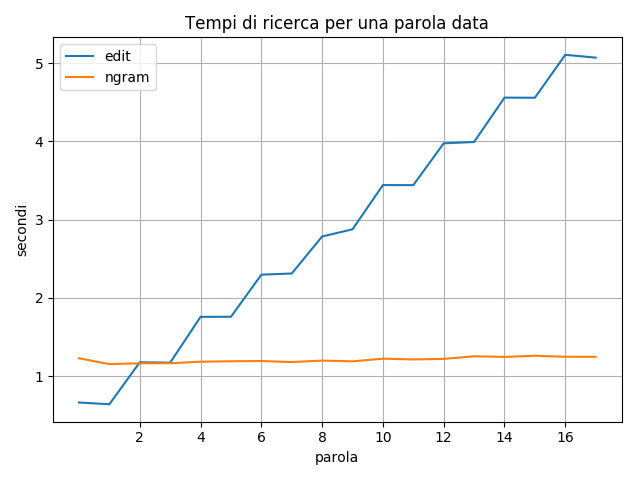
\includegraphics[width=1.0\textwidth]{Tempi_di_ricerca_per_una_parola_data}
    \caption{Tempo di esecuzione di Edit Distance e N-grammi per parole di dimensione variabile.}
    \label{fig:test2_1}
\end{figure}
Per questo esperimento sono state prese 18 parole arbitrarie di lunghezza crescente dall'elenco di parole italiane ($60000\_parole\_italiane.txt$): 'a', 'c', 'ad', 'ed', 'con', 'dal', 'muro', 'cane', 'zoppo', 'gatto', 'marito', 'pulito', 'sboccia', 'cantare', 'faticavo', 'fratelli', 'penzolano', 'cameriere'.
\newline
\newline
Per ognuna delle parole scelte è stato applicato sia l'algoritmo di Edit Distance che N-grammi.
\newline
\newline
Dal grafico si può notare che il tempo dell'algoritmo N-grammi è quasi costante ($\sim 3  secondi$) qualsiasi sia la lunghezza della parola.
\newline
\newline
I tempi dell'Edit Distance, al contrario, crescono in maniera lineare all'aumentare della lunghezza della parola scelta.
\newline
\newline
In conclusione, se si ha a che fare con parole lunghe, l'algoritmo di N-grammi è nettamente più efficiente.

\clearpage
\subsection{Numero di parole vicine trovate con Edit Distance e N-grammi per parole di dimensione variabile}
\begin{figure}[h]
    \centering
    \captionsetup{justification=centering,margin=1.05cm}
    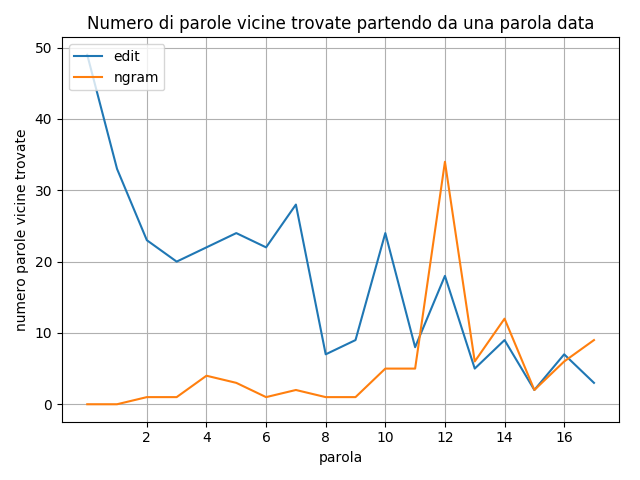
\includegraphics[width=1.0\textwidth]{Figure_2}
    \caption{Numero di parole vicine trovate con Edit Distance e N-grammi per parole di dimensione variabile.}
    \label{fig:test2_2}
\end{figure}
Anche per questo esperimento sono state prese 18 parole arbitrarie di lunghezza crescente dall'elenco di parole italiane ($60000\_parole\_italiane.txt$): 'a', 'c', 'ad', 'ed', 'con', 'dal', 'muro', 'cane', 'zoppo', 'gatto', 'marito', 'pulito', 'sboccia', 'cantare', 'faticavo', 'fratelli', 'penzolano', 'cameriere'.
\newline
\newline
Per ognuna delle parole scelte è stato applicato sia l'algoritmo di Edit Distance che N-grammi.
\newline
\newline
Dal grafico si può notare che il numero di parole vicine trovate dell'algoritmo N-grammi è crescente, con il crescere della lunghezza della parola.
\newline
\newline
Il numero di parole trovate da Edit Distance, al contrario, decrescono all'aumentare della lunghezza della parola scelta.

\clearpage
\subsection{Numero di risultati trovati al variare della soglia di $Edit$ $distance$}
\begin{figure}[h]
    \centering
    \captionsetup{justification=centering,margin=1.05cm}
    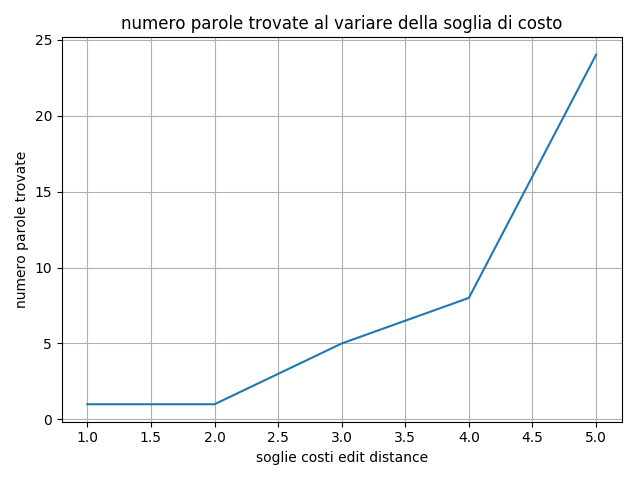
\includegraphics[width=1.0\textwidth]{Figure_3_2}
    \caption{Numero di parole vicine ad una parola data ( 'promosso' ) al variare della soglia di $Edit$ $distance$}
    \label{fig:test3_1}
\end{figure}
Per questo esperimento è stata presa in ingresso una parola chiesta all'utente, in questo caso 'promosso', alla quale è stato applicato l'algoritmo $Edit$ $distance$ più volte.
\newline
\newline
Per ogni volta che viene applicato $Edit$ $distance$ la soglia di errore viene aumentata di 1, per osservare come varia l'insieme di parole restituite dall'algoritmo.
\newline
\newline
Dal grafico si può notare che il numero di parole vicine trovate dell'algoritmo $Edit$ $distance$ sia proporzionale all'aumento della soglia di $Edit$ $distance$.
\newline
\newline

\clearpage
\subsection{Numero di risultati trovati al variare del coefficiente di Jaccard}
\begin{figure}[h]
    \centering
    \captionsetup{justification=centering,margin=1.05cm}
    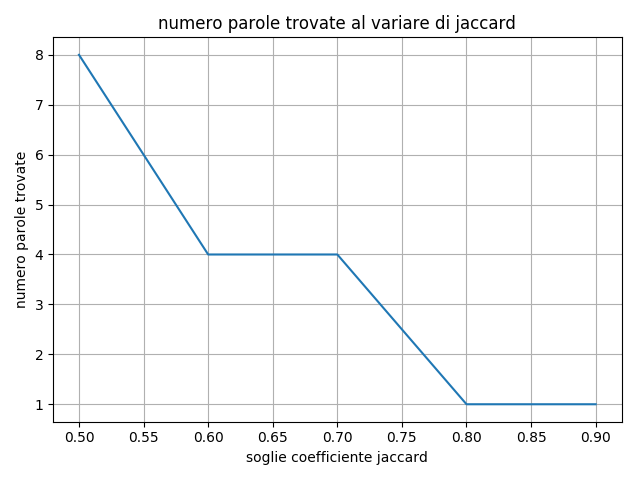
\includegraphics[width=1.0\textwidth]{Figure_3_1}
    \caption{Numero di parole vicine ad una parola data ( 'promosso', ) al variare della soglia di $Edit$ $distance$}
    \label{fig:test3_2}
\end{figure}
Anche per questo esperimento è stata presa in ingresso una parola chiesta all'utente, in questo caso 'promosso', alla quale è stato applicato l'algoritmo $N-gram$ più volte.
\newline
\newline
Per ogni volta che viene applicato $N-gram$ il coefficiente di Jaccard vine aumentato di 0.1, per osservare come varia l'insieme di parole restituite dall'algoritmo.
\newline
\newline
Dal grafico si può notare che il numero di parole vicine trovate dell'algoritmo $N-gram$ sia inversamente proporzionale all'aumento del coefficiente di Jaccard.
\newline
\newline

\clearpage
\subsection{Numero di parole vicine trovate al variare del numero di N-grammi}
\begin{figure}[h]
    \centering
    \captionsetup{justification=centering,margin=1.05cm}
    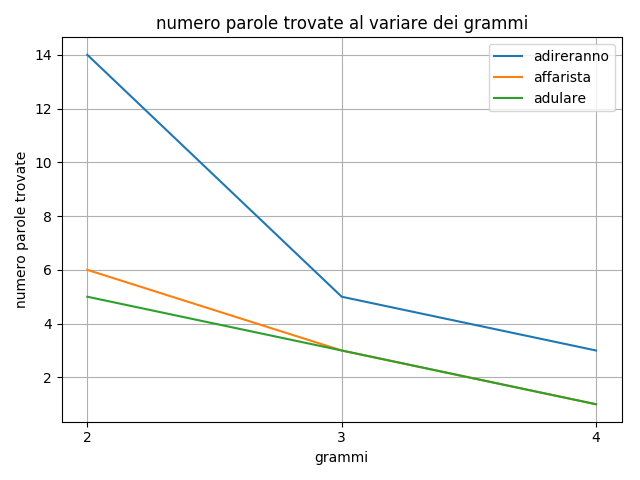
\includegraphics[width=1.0\textwidth]{Figure_4}
    \caption{Numero di parole vicine a parole casuali trovate utilizzando bi-grammi, trigrammi e quadrigrammi}
    \label{fig:test4_1}
\end{figure}
Per questo esperimento sono state utilizzate tre parole casuali ( 'adireranno', 'affarista', 'adulare'), alle quali è stato applicato l'algoritmo $N-gram$ più volte.
\newline
\newline
Per ogni volta che viene applicato $N-gram$ si utilizza diversi valori di $n$, in particolare [2, 3, 4].
\newline
\newline
Dal grafico, e da molteplici esperimenti eseguiti, si nota come il numero di parole trovate non dipenda dal valore di $n$, ma varia ogni volta a seconda della parola scelta e della sua lunghezza.
\newline
z
\clearpage
\subsection{Risultati della ricerca di una parola alterata tramite Edit distance e N-gram al variare della soglia e del coefficiente di jaccard.}

Per questo esperimento è stata presa in ingresso una parola chiesta all'utente, in questo caso 'ventisette' sulla quale è stata eseguita un'alterazione casuale tra le tre possibili :
\newline
-Scambio di due caratteri casuali \newline
-Eliminazione di un carattere casuale \newline
-Aggiunta di un carattere casuale \newline
\newline
In questo caso la parola 'ventisette' è stata alterata tramite uno scambia di caratteri in 'ventisetet'.
\newline
\begin{center}
\vspace*{0.7cm}
\begin{tabular}{|c|c|c|}
\hline
\textbf{Soglia di costo}\bigstrut & \textbf{Parola originale trovata}  & \textbf{Parole vicine trovate} \\ \hline
 1\bigstrut & no & 0 \\\hline
 2\bigstrut & si & 1 \\\hline
 3\bigstrut & si & 1 \\\hline
 4\bigstrut & si & 2 \\\hline
 5\bigstrut & si & 7 \\\hline
\end{tabular}
\captionsetup{justification=centering,margin=1.05cm}
\captionof{table}{Tabella che mostra i risultati dell'esperimento al variare della soglia di costo di $Edit$ $distance$.}
\end{center}

\begin{center}
\vspace*{0.7cm}
\begin{tabular}{|c|c|c|}
\hline
\textbf{Coefficiente di Jaccard}\bigstrut & \textbf{Parola originale trovata}  & \textbf{Parole vicine trovate} \\ \hline
 0.5\bigstrut & si & 3 \\\hline
 0.6\bigstrut & si & 2 \\\hline
 0.7\bigstrut & si & 1 \\\hline
 0.8\bigstrut & si & 1 \\\hline
 0.9\bigstrut & si & 1 \\\hline
\end{tabular}
\captionsetup{justification=centering,margin=1.05cm}
\captionof{table}{Tabella che mostra i risultati dell'esperimento al variare del coefficiente di Jaccard.}
\end{center}
Dalle tabelle, e da molteplici esperimenti eseguiti, si nota che generalmente la parola originale è ritrovata più volte tramite $Edit$ $distance$, rispetto ad $N-gram$, anche con soglie di errore alte.
\newline
\newline
Questo fatto però non è sempre vero, infatti la possibilità di ritrovare la parola originaria, sia con $Edit$ $distance$ sia con $N-gram$, dipende dalla parola scelta, dal tipo di alterazione e dalla parte specifica di parola che viene alterata.
\clearpage

\section{Conclusioni}
In conclusione, come ci si aspettava dalla teoria, gli esperimenti hanno evidenziato differenze tra Edit Distance e N-grammi.

Infatti per quanto riguarda i \textbf{tempi di esecuzione}, Edit Distance si è effettivamente rivelato più lento rispetto agli N-grammi in quanto deve eseguire molti più confronti.
\newline
Questo infatti è evidenziato soprattutto nella ricerca di parole 'lontane' dall'inizio del vocabolario, per le quali il tempo di ricerca di Edit distance supera di gran lunga quello di N-gram per la stessa parola, proprio per la gran differenza di operazioni eseguite sulle singole parole.
\newline
Per quanto riguarda il \textbf{numero di parole vicine trovate}, la situazione è capovolta:
Edit distance riesce, generalmente, a trovare molte parole vicine ad una parola data, anche con soglie di errore alte, mentre N-gram trova quasi sempre un numero minore di parole vicine.
\newline
Questa differenza è dovuta sopratutto al coefficiente dei costi sul quale si basa Edit distance, nel nostro caso il costo della copia di un caratere era nulla, e ciò permette ad Edit distance di trovare le parore molto simili ad una data anche soglie di errore alta.
\newline
Dagli esperimenti svolti è possibile ritenere che la funzione Edit distance sia da preferirsi ad N-gram per la realizzazione di un correttore ortografico, poichè generalmente riesce a ritrovare più facilmente la parola originale.

\end{document}
